\chapter{Other low-energy physics with P-type point contact detectors}

In this section, we basically discuss two things: Heavy non-relativistic axions, the signal, and the exclusion limit as calculated with the data from the previous chapter.

Also, making some reasonable assumptions about Majorana, we make some estimates as to the sensitivity of the Majorana experiment to WIMP dark matter and axion dark matter (via the axioelectric effect).  

		
	\section{Other dark matter: heavy axions}
	\label{sec:CalcLimitsOnHeavyAxions}		
		


	\subsection{Heavy axion signal}
	\label{sec:CalcLimitsOnHeavyAxionSignal}		

	The signal for a non-relativistic axion interacting via the axioelectric effect has been derived in~\cite{Pospelov:2008jk}.  This particular inelastic interaction involves the deposition of the \emph{complete} energy of the axion which, in the non-relativistic case, is essentially equal to the mass of the particle.  Since the excitation of the electron via the axioelectric effect is similar to that mediated by a photon in the photoelectric effect, the signal is a delta function centered at the mass of the axion, $m_{a}$.  Convolved with the detector resolution, the signal would appear gaussian with width exactly that of a gamma or x-ray of energy equivalent to $m_{a}$.  The rate of this interaction has been estimated in~\cite{Pospelov:2008jk} as:
	
		\begin{equation}
			R \left[ kg^{-1} day^{-1} \right]\simeq \frac{1.2\times 10^{19}}{A} \gaa^{2} m_a \sigma_{photo}
			\label{eqn:AxioelectricRate}
		\end{equation}

where $A$ is the atomic mass, $m_{a}$ is the mass of the axion in keV, $\sigma_{photo}$ is the measured photoelectric cross section in barns, and $g_{a\bar{e}e}$ is the dimensionless coupling constant.  In the derivation of this result, the value of the density of the dark matter $\rho_{D}$ = 0.3~GeV cm$^{-3}$ was used.  The rate calculated for a germanium detector ($A=72.96$) with a chosen coupling constant, $\gaa = 10^{-11}$, is given in Figure~\ref{fig:HeavyAxionSignalRate}.  The rate calculation used well-known cross sections obtained from the NIST FFAST database located online~\cite{chantler:597}.  

The low noise of PPC detectors yields excellent sensitivity to non-relativistic axions with masses $\leq10$~keV due their sharp resolution at low energies.  A comparison of an axioelectric signal at a given $\gaa$ is provided in Figure~\ref{fig:ResCompare} for characteristic resolutions of NaI and germanium detectors.  In this plot, it is clear that the improved resolution of the germanium detector allows less smearing of the signal, forcing more counts into a narrower peak.

		\begin{figure}
			\centering
			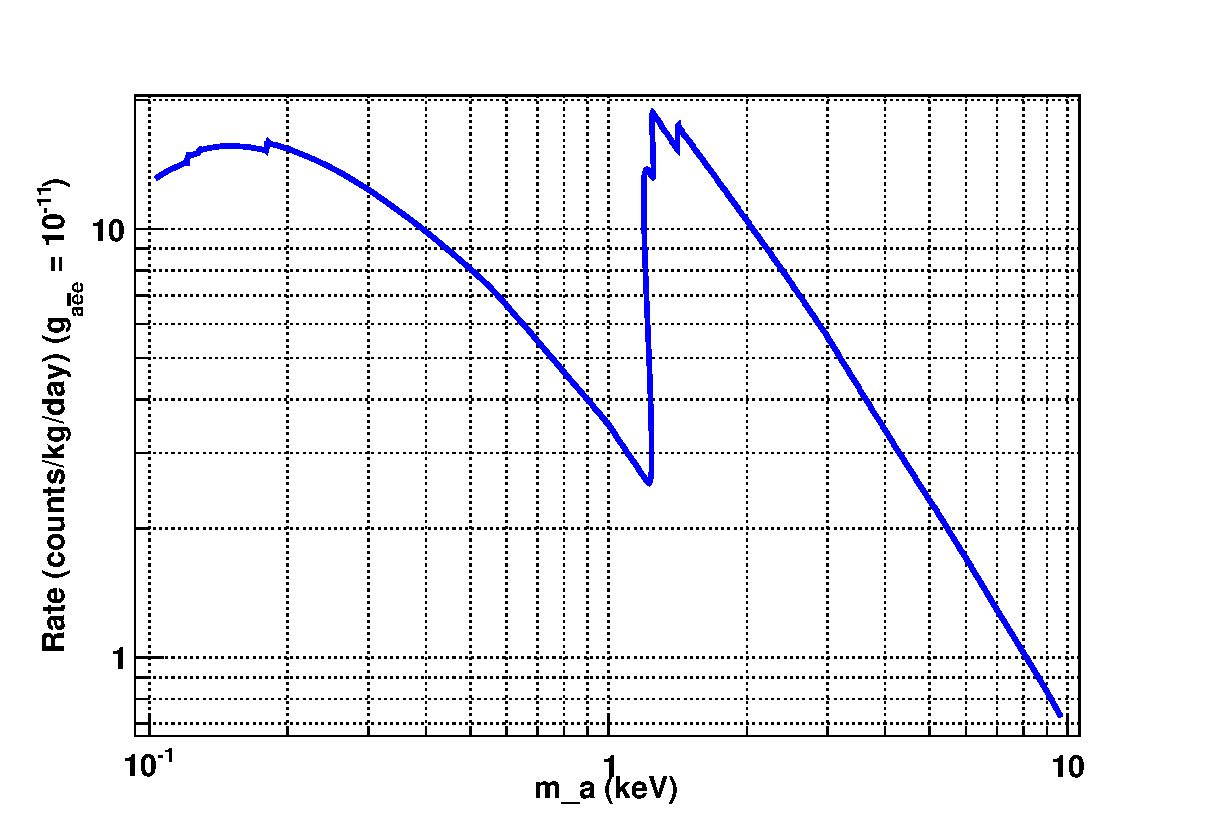
\includegraphics[width=0.9\textwidth]{GeRate}
			\caption[Axioelectric interaction rate in germanium]{Non-relativistic axion axioelectric 
			interaction rate in germanium.  The photoelectric cross section for germanium was obtain
			from the NIST database~\cite{chantler:597}.}
			\label{fig:HeavyAxionSignalRate}
		\end{figure}

		\begin{figure}
			\centering
			\includegraphics[width=0.9\textwidth]{DAMARes}
			\caption[Axion signal at $m_{a}$ = 3.2~keV]{Axion signal at $m_{a}$ = 3.2~keV comparing 
			the detector responses of germanium (blue, dashed) and NaI (red, solid) to an equivalent
			$\gaa$.  }
			\label{fig:ResCompare}
		\end{figure}

	\subsection{Limits on the axioelectric effect}
	\label{sec:CalcLimitsOnHeavyAxionLimits}		
		
	Limits were calculated using the profile-likelihood method described in Section~\ref{sec:LimitsML}.  Fit were performed on the complete number of data sets described in Chapter~\ref{chap:AnalysisBeGe}, but all data sets yielded similar results and so one data set was chosen with 95\% rise-time acceptance cuts and microphonics cuts applied.  The difficulties seen while determining limits on low-mass WIMPs did not appear in these calculations because the signal (gaussian centered at $m_{a}$) was not in general similar to the background.  The limit calculation followed the same procedure as a peak search in the data and is outlined as follows:
		\begin{itemize}
			\item Define the gaussian signal $f_{axion}$: 
			\begin{itemize}
				\item Choose mass $m_{a}$ of the axion defining $\mu$ of gaussian
				\item Determine $\sigma$ at $E = m_{a}$ using resolution in Equation~\ref{eqn:SigmaEqn}.
			\end{itemize}
			\item Fit to the function $B + N_{axion} f_{axion}$ where $B$ is the background defined in Section~\ref{sec:LimitsDataAndModel} and determine the profile likelihood $\plln$.
			\item Determine the 90\% upper limit on $N_{axion}$ using $\plln$.
			\item Repeat for other values of $m_{a}$
		\end{itemize}		
	
	During the fits, the $\mu$ and $\sigma$ of the gaussian signal, $f_{axion}$, were kept fixed and only the amplitude, $N_{axion}$ was kept as a free parameter of the signal.  For the background, the behavior of the parameters was the same as during WIMP exclusion fits (see Section~\ref{sec:LimitsDataAndModel}) and the relative amplitude of the \gersixeight~and\znsixfive~L-lines was kept fixed as described in Section~\ref{sec:LimitsConstrained}.  Fixing this relative amplitude served to minimize the impact of the L-lines in the exclusion fits since a signal centered at 1.1 and 1.3~keV will look exactly like the L-capture lines.  The value of the axion mass was scanned from 0.1~keV to 7.8~keV in steps of 0.2~keV using both high- and low-gain channels: high-gain channel, $0.1\to2.9$~keV; low-gain channel, $3\to7.8$~keV.  

		\begin{figure}
			\centering
			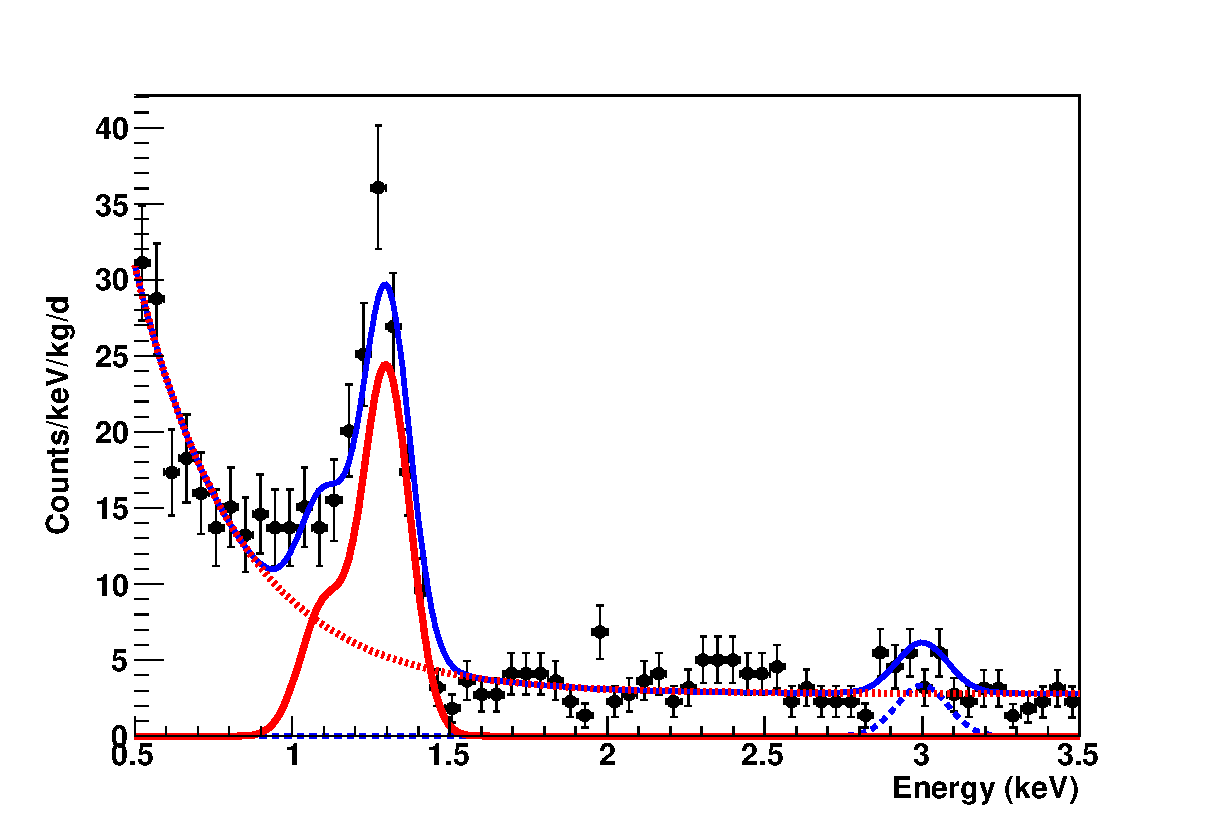
\includegraphics[width=0.9\textwidth]{AxioelectricFitExample}
			\caption[Example of an excluded non-relativistic axioelectric signal at $m_{a}=3$~keV at 
			90\% CL]{Example of an excluded non-relativistic axioelectric signal at $m_{a}=3$~keV at 
			90\% CL.  In this fit, $N_{axion}$ is 36.1 counts.  The components of the fits are noted}
			\label{fig:ExampleHeavyAxionFit}
		\end{figure}
			
		\begin{figure}
			\centering
			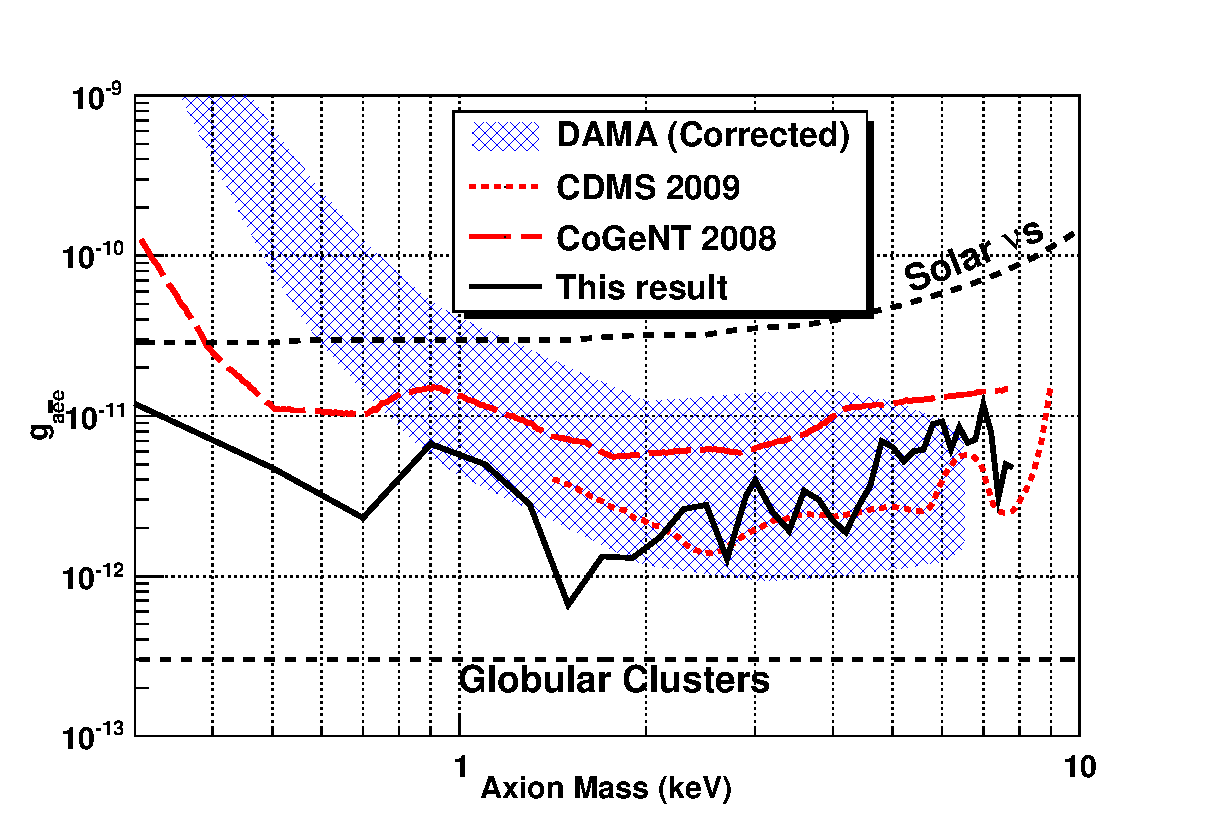
\includegraphics[width=0.9\textwidth]{axion_constrained_unbinnedall_exclusion_plots_final}
			\caption{Limits on non-relativistic axions.}
			\label{fig:HeavyAxionLimits}
		\end{figure}
		

							
	\section{Sensitivity of the \MJ~\minmod~to a Dark Matter signal}
	\label{sec:MJSensitivity}
	
		\subsection{Low-energy background model}
		\label{sec:MJLowEnergyBackgroundModel}
		
		\subsection{WIMPs}
		\label{sec:MJSensitivityToWIMP}
		
			\begin{figure}
				\centering
				%\includegraphics[width=0.9\textwidth]{PPC2DesignSchematicAll}
				\caption{\MJ~\minmod~sensitivity to a WIMP signal.}
				\label{fig:MJSensitivityToWIMP}
			\end{figure}		
			
		\subsection{Heavy axions}
		\label{sec:MJSensitivityToAxions}
		
			\begin{figure}
				\centering
				%\includegraphics[width=0.9\textwidth]{PPC2DesignSchematicAll}
				\caption{\MJ~\minmod~sensitivity to a Heavy Axion signal.}
				\label{fig:MJSensitivityToHeavyAxions}
			\end{figure}							

	\section{Conclusions}
	\label{sec:OtherLowEnergyConclusions}	